% !TEX program = pdflatex
\documentclass[11pt]{article}

\usepackage[a4paper,margin=2.4cm]{geometry}
\usepackage{amsmath,amssymb,amsthm,mathtools}
\usepackage{graphicx}
\usepackage{booktabs}
\usepackage{enumitem}
\usepackage[hidelinks]{hyperref}
\usepackage{microtype}
\usepackage{subcaption}

\theoremstyle{plain}
\newtheorem{theorem}{Theorem}[section]
\newtheorem{lemma}[theorem]{Lemma}
\newtheorem{proposition}[theorem]{Proposition}
\newtheorem{corollary}[theorem]{Corollary}
\theoremstyle{definition}
\newtheorem{definition}[theorem]{Definition}
\newtheorem{conjecture}[theorem]{Conjecture}
\theoremstyle{remark}
\newtheorem{remark}[theorem]{Remark}

\newcommand{\Ez}{\mathbb{Z}}
\newcommand{\Floor}[1]{\left\lfloor #1\right\rfloor}
\newcommand{\Ceil}[1]{\left\lceil #1\right\rceil}
\newcommand{\pack}{\mathcal{P}}
\newcommand{\triangles}{\mathcal{T}}

\title{\bfseries Edge-disjoint non-crossing triangle packings of planar point sets:\\
a convex barrier and a reduction to subcubic trees}
\author{Rajveersinh Pardeshi}
\date{}

\begin{document}
\maketitle

\begin{abstract}
Given a finite set $P$ of points in general position in the plane, let $\nu(P)$ be the
largest size of a family of triangles spanned by $P$ such that no two triangles share an
edge and no edge of one triangle crosses an edge of another.  We determine $\nu$ exactly
when $P$ is in convex position: it equals $\Floor{(2n-3)/3}$ for $|P|=n$.  The main
structural observation is that in convex position the problem is purely combinatorial:
every $3$-cycle of a triangulation of a convex polygon bounds a face, so $\nu(P)$ equals
the independence number of the weak dual of some triangulation, and every subcubic tree
occurs as such a weak dual.  Consequently the convex extremal function is exactly the
maximum independence number of a subcubic tree, which is $\Floor{(2N+1)/3}$.  For
arbitrary point sets we prove the sharp bound $\nu(P)\le n-2$ and determine when it is
attained: for maximal planar graphs the bound is attained exactly by the Eulerian ones,
and Eulerian triangulations exist precisely for $n\in\{3\}\cup\{n\ge 6: n\ne 7\}$.  We
conjecture that convex position is the worst configuration, i.e.\
$\nu(P)\ge\Floor{(2n-3)/3}$ for every $n$-point set, with equality only in convex
position.  We were unable to prove this and report a search for counterexamples instead.
\end{abstract}

\section{Introduction}

Let $P$ be a finite set of points in general position in the plane.  Call a family
$\pack$ of $3$-element subsets of $P$ a \emph{packing} if no two members share two points
and no edge of one member crosses an edge of another; let $\nu(P)$ be the maximum size of
a packing, and put
\[
f(n)\;=\;\max\{\nu(P): |P|=n,\ P\text{ in convex position}\}.
\]

Condition one is a packing condition on edges; condition two says the union of the
triangles is a plane straight-line graph.  Together they interpolate between two classical
themes: packing edge-disjoint copies of a graph inside a planar graph, and extremal
questions about the complete geometric graph on $n$ points.

The paper has three parts.

\begin{enumerate}
\item \textbf{Convex position.}  We prove
  \[
  f(n)=\Floor{(2n-3)/3}\qquad(n\ge 3),
  \]
  and give an explicit construction attaining it.  The upper bound is a two-line edge
  count; the content is the construction and the identification below.
\item \textbf{A tree reduction.}  In convex position the problem is exactly a problem
  about independence numbers of trees.  If $a(N)$ is the maximum independence number of a
  tree on $N$ vertices of maximum degree at most $3$ (``subcubic''), then
  \[
  f(n)=a(n-2),\qquad a(N)=\Floor{(2N+1)/3}\quad(N\ge 1).
  \]
  The second identity has a two-line proof (a vertex-cover count) and a matching explicit
  construction.
\item \textbf{Arbitrary point sets.}  We prove $\nu(P)\le n-2$ and, for maximal planar
  graphs, determine exactly when that bound is attained: precisely for the Eulerian ones.
  Eulerian triangulations exist exactly for $n\in\{3\}\cup\{n\ge 6: n\ne 7\}$.
\end{enumerate}

Part 2 is mildly surprising: the convex extremal function of a problem that looks
geometric coincides, term by term, with the maximum independence number of a subcubic
tree.  Part 3 explains why convex position is the \emph{hardest} configuration rather than
the easiest: the union of a packing is always a plane graph, but in convex position that
plane graph is forced to be outerplanar, which costs roughly a quarter of the available
edges.

The natural remaining question is Conjecture~\ref{conj:barrier}: whether convex position is
really the worst configuration.  We do not prove it, and we say so.

\section{Related work and novelty}

\paragraph{Packing plane spanning objects.}
There is an active literature on packing edge-disjoint plane spanning trees and paths in a
point set \cite{aichholzer2017}.  Those objects have $n-1$ edges each, so a counting
argument and an explicit family settle the extremal question.  Our objects are triangles,
with $3$ edges each, and the constraint is edge-disjointness together with non-crossing
rather than spanningness.  The closely related \emph{book thickness} of $K_n$ also yields
$\Ceil{n/2}$ \cite{bernhartkainen1979}; that is a different problem (pages along a common
Hamiltonian path), and we mention it only to say that our numerical value
$\Floor{(2n-3)/3}$ coincides with no such classical quantity.

\paragraph{Convex geometric hypergraphs.}
A substantial literature studies $k$-uniform convex geometric hypergraphs under Tur\'an-type
and saturation conditions \cite{furedijiangkostochka2020,oneillspiro2021}.  There the
objects of study are families of convex $k$-gons subject to a forbidden configuration, and
no non-crossing constraint is imposed on the family itself.  Our problem is the
complementary one: the forbidden configuration is the family of all crossings.

\paragraph{Eulerian triangulations.}
The equivalence between Eulerian triangulations of the sphere and cubic bipartite planar
graphs is classical.  The existence question used in Part 3 is an elementary instance of
it, treated in Lemma~\ref{lem:exists}.

\paragraph{Novelty.}
We did not find a published result establishing $f(n)=\Floor{(2n-3)/3}$ for edge-disjoint
non-crossing triangle packings of a convex $n$-gon.  We searched under the terminology
``edge-disjoint triangles'', ``non-crossing triangles'', ``triangle packing'', ``convex
position'', ``outerplanar graph'', ``maximal outerplanar graph'', ``weak dual'' and
``independence number of a subcubic tree'', and also consulted the nearest neighbour
literature above.  We also did not find the identity $f(n)=a(n-2)$, which removes geometry
from the convex case entirely, nor the characterisation in Part 3.  We make no priority
claim beyond this, and Conjecture~\ref{conj:barrier} is labelled a conjecture precisely
because we cannot prove it.

\section{Definitions and preliminaries}

\begin{definition}[Packing]\label{def:packing}
Let $P$ be a finite point set in general position in the plane.  A \emph{packing} of $P$
is a family $\pack\subseteq\binom{P}{3}$ such that
\begin{enumerate}[label=(\roman*)]
\item $|A\cap B|\le 1$ for all distinct $A,B\in\pack$;
\item the relative interiors of an edge of $A$ and an edge of $B$ are disjoint for all
      distinct $A,B\in\pack$.
\end{enumerate}
$\nu(P)$ denotes the maximum size of a packing of $P$.
\end{definition}

\begin{definition}[Convex position]\label{def:convexpos}
$P$ is in \emph{convex position} if every point of $P$ is a vertex of $\operatorname{conv}(P)$,
i.e.\ $P$ is the vertex set of a convex polygon.  Write $f(n)$ for the largest value of
$\nu(P)$ over such sets with $|P|=n$.
\end{definition}

\begin{lemma}[Edge counts]\label{lem:edges}
Let $P$ be an $n$-point set in general position, $\pack$ a packing of $P$ of size $t$, and
$G$ the union of the edges of the triangles in $\pack$.
\begin{enumerate}[label=(\alph*)]
\item[(a)] If $P$ is in convex position then $|E(G)|\le 2n-3$, so
      $t\le\Floor{(2n-3)/3}$.
\item[(b)] In general $|E(G)|\le 3n-6$, so $t\le n-2$.
\end{enumerate}
\end{lemma}

\begin{proof}[(a)]
$G$ is drawn with straight segments inside $\operatorname{conv}(P)$ and no two of its edges
cross.  Every point of $P$ is a vertex of the polygon $\operatorname{conv}(P)$, hence every
vertex of $G$ lies on the outer face of $G$; thus $G$ is outerplanar and $|E(G)|\le 2n-3$.
By condition (i) of Definition~\ref{def:packing} the $t$ triangles contribute $3t$
distinct edges, so $3t\le 2n-3$.
\end{proof}

\begin{proof}[(b)]
$G$ is planar with at most $n$ vertices, so $|E(G)|\le 3n-6$ and $3t\le 3n-6$.
\end{proof}

\begin{remark}\label{rem:outerplanar}
Lemma~\ref{lem:edges}(a) is why convex position is expected to be the hardest
configuration: the union of a packing is forced to be outerplanar there, which costs about
a quarter of the edges compared with the planar bound of Lemma~\ref{lem:edges}(b).
\end{remark}

\begin{definition}[Triangulation and weak dual]\label{def:tri}
A \emph{triangulation} $T$ of a convex $n$-gon is a maximal non-crossing set of
diagonals; equivalently, a maximal outerplanar graph whose outer face is the polygon cycle.
It has $n-2$ triangular faces and $2n-3$ edges.  Its \emph{weak dual} $D(T)$ has one
vertex per triangular face and one edge per pair of faces sharing an edge; $D(T)$ is a tree
on $n-2$ vertices of maximum degree at most $3$.
\end{definition}

\begin{lemma}[Every subcubic tree occurs]\label{lem:subcubic}
For $N\ge 1$ the weak duals of triangulations of the convex $(N+2)$-gon are exactly the
trees on $N$ vertices of maximum degree at most $3$.
\end{lemma}

\begin{proof}
One direction: a face of a triangulation has three sides, so $\Delta(D(T))\le 3$; and
$D(T)$ is a tree, since the faces of a polygon triangulation are connected through the
$n-3$ shared diagonals, giving a connected graph on $n-2=N$ vertices with $N-1$ edges.

For the converse let $S$ be a tree on $N$ vertices with $\Delta(S)\le 3$, rooted at $r$.
Take $N$ abstract triangles and glue them according to $S$: glue the triangle of $v$ to
the triangle of $\operatorname{parent}(v)$ along one side of each.  Since $S$ is a tree, no
side is demanded twice, and $\Delta(S)\le 3$ guarantees that no triangle is asked for more
than three sides.  The result is a triangulated disc with $3+(N-1)=N+2$ vertices, all on
its boundary, and with $3+2(N-1)=N+2$ boundary edges; it is therefore a maximal outerplanar
graph.  Every maximal outerplanar graph is combinatorially the graph of a triangulation of
a convex polygon (place the vertices on a circle in the order of the outer face), and by
construction its dual tree is $S$.
\end{proof}

\begin{lemma}[Threecycles are faces]\label{lem:faces}
Let $T$ be a triangulation of a convex $n$-gon and let $\Delta$ be a $3$-cycle of the graph
of $T$.  Then $\Delta$ bounds a face of $T$.  Consequently the largest number of pairwise
edge-disjoint triangles of $T$ equals $\alpha(D(T))$.
\end{lemma}

\begin{proof}
No vertex of a point set in convex position lies strictly inside a triangle spanned by
three of its vertices, since such a vertex would not be a vertex of the convex hull.
Suppose $\Delta$ were not a face.  Then some edge $e$ of $T$ lies strictly inside $\Delta$
and the two faces of $T$ incident with $e$ lie inside $\Delta$.  At least one endpoint of
$e$ is not a vertex of $\Delta$ (otherwise $e$ would be a side of $\Delta$), and that
endpoint lies strictly inside $\Delta$, a contradiction.  Finally, two faces of $T$ share an
edge exactly when the corresponding vertices of $D(T)$ are adjacent, so pairwise
edge-disjoint faces are exactly independent sets of $D(T)$.
\end{proof}

\begin{lemma}[When a polygon triangulation is determined combinatorially]\label{lem:poly}
The combinatorics of a triangulation of a convex $n$-gon depend only on $n$: any maximal
outerplanar graph is the graph of a triangulation of some convex polygon.
\end{lemma}

\begin{proof}
Let $M$ be a maximal outerplanar graph and let the boundary cycle of one of its outerplane
embeddings be $v_1v_2\cdots v_m$.  Place $m$ points on a circle in the order
$v_1,\dots,v_m$.  Each edge of $M$ is a chord of this polygon; two chords of a circle cross
in their relative interiors if and only if their four endpoints alternate around the circle.
If two edges of $M$ crossed in the outerplane embedding they would lie in disjoint faces of
$M$ bounded by chords of the boundary cycle, forcing two of their endpoints to alternate,
contradiction.  Hence the circle drawing is planar and is a triangulation of the
$m$-gon.  (This is the usual identification of maximal outerplanar graphs with polygon
triangulations.)
\end{proof}

\section{Convex position: the exact answer}

\begin{theorem}\label{thm:f}
For every $n\ge 3$, $\;f(n)=\Floor{(2n-3)/3}$.
\end{theorem}

Lemma~\ref{lem:edges}(a) gives the upper bound, so it remains to construct packings of that
size.  Lemma~\ref{lem:faces} lets us choose the triangulation first and then look for a
large independent set in its weak dual.

\begin{proposition}[The recurrence]\label{prop:rec}
Fix $i<j$ and write $P(i,j)=(v_i,v_{i+1},\dots,v_j)$.  Let $\Phi(i,j)$ be the largest
number of pairwise edge-disjoint triangles of a triangulation of $P(i,j)$, maximised over
triangulations; and let $\Psi(i,j)$ be the same maximum restricted to triangulations in
which the chord $(v_i,v_j)$ is used by no triangle.  Then
\begin{align}
\Phi(i,j)&=\max_{i<k<j}\max\bigl\{\Phi(i,k)+\Phi(k,j),\;1+\Psi(i,k)+\Psi(k,j)\bigr\},
\label{eq:rec}\\
\Psi(i,j)&=\max_{i<k<j}\bigl\{\Phi(i,k)+\Phi(k,j)\bigr\}.
\label{eq:rec1b}
\end{align}
\end{proposition}

\begin{proof}
Let $T$ be a triangulation of $P(i,j)$ and let $(v_i,v_k,v_j)$ be the face of $T$ incident
with the chord $(v_i,v_j)$; it exists and is unique because that chord is a boundary edge
of $P(i,j)$.  The chords $(v_i,v_k)$ and $(v_k,v_j)$ cut $P(i,j)$ into $P(i,k)$ and
$P(k,j)$.  By Lemma~\ref{lem:faces} every $3$-cycle of $T$ is a face of $T(i,k)$, a face of
$T(k,j)$, or the face $(v_i,v_k,v_j)$ itself: a $3$-cycle meeting both sides would have to
contain one of the two cutting chords as a side, in which case it is the root face.  The
two sub-triangulations share no edge (they meet only in $v_k$), so their packings combine
freely.

If the root face is not chosen, the packing splits into a packing of $T(i,k)$ and one of
$T(k,j)$; nothing uses $(v_i,v_j)$, which gives the first term of $\Phi$ and the whole of
$\Psi$.  If the root face is chosen, the chords $(v_i,v_k)$ and $(v_k,v_j)$ are consumed,
so both sub-packings are $\Psi$-constrained; this gives the second term of $\Phi$, and it is
inadmissible in $\Psi$ because the root face uses $(v_i,v_j)$.
\end{proof}

By Lemma~\ref{lem:poly} the values of $\Phi$ and $\Psi$ depend only on the number $m$
$j-i+1$ of vertices.  Writing $\phi_m,\psi_m$ for them, \eqref{eq:rec} becomes
\begin{equation}\label{eq:rec2}
\phi_m=\max_{\substack{a,b\ge 2\\ a+b=m+1}}\max\{\phi_a+\phi_b,\;1+\psi_a+\psi_b\},
\qquad
\psi_m=\max_{\substack{a,b\ge 2\\ a+b=m+1}}\{\phi_a+\phi_b\},
\end{equation}
with $\phi_0=\phi_1=\psi_0=\psi_1=\phi_2=\psi_2=0$.

\begin{lemma}\label{lem:closed}
For all $m\ge 3$, $\;\phi_m=\Floor{(2m-3)/3}$ and $\psi_m=\Floor{(2m-4)/3}$.
\end{lemma}

\begin{proof}
Strong induction on $m$.  For $m\le 5$ one reads off \eqref{eq:rec2} by hand:
$\phi_3=1,\ \phi_4=1,\ \phi_5=2$ and $\psi_2=0,\ \psi_3=0,\ \psi_4=1,\ \psi_5=2$.

\emph{Bound for $\psi$.} Let $m\ge 5$ and let $a$ be the largest multiple of $3$ with
$a\le m-1$; put $b=m+1-a$, so $b\in\{2,3,4\}$ and $b\ge 2$.  Then
\begin{equation*}
\psi_m\;\ge\;\phi_a+\phi_b\;\ge\;
\Bigl\lfloor\tfrac{2a-3}{3}\Bigr\rfloor+\Bigl\lfloor\tfrac{2b-3}{3}\Bigr\rfloor
\;\ge\;\Bigl\lfloor\tfrac{2a+2b-6}{3}\Bigr\rfloor
\;=\;\Bigl\lfloor\tfrac{2m-4}{3}\Bigr\rfloor,
\end{equation*}
the third step using $3\mid a$, so that $(2a-3)/3$ is an integer and the two floors add
without loss.

\emph{Bound for $\phi$.} Let $m\ge 5$ and let $a$ be the largest integer with
$a\equiv 2\pmod 3$ and $a\le m-1$; then $2a-4\equiv 0 \pmod 3$ and, with
$b=m+2-a$ (so $2\le b\le 4$), the ``root face chosen'' branch of \eqref{eq:rec2} applies and
gives, by induction,
\begin{equation*}
\phi_m\;\ge\;1+\psi_a+\psi_b\;\ge\;
1+\Bigl\lfloor\tfrac{2a-4}{3}\Bigr\rfloor+\Bigl\lfloor\tfrac{2b-4}{3}\Bigr\rfloor
\;\ge\;1+\Bigl\lfloor\tfrac{2a+2b-8}{3}\Bigr\rfloor
\;=\;1+\Bigl\lfloor\tfrac{2m-6}{3}\Bigr\rfloor
\;=\;\Bigl\lfloor\tfrac{2m-3}{3}\Bigr\rfloor .
\end{equation*}

For the reverse inequalities: $\psi_m\le\phi_m$ and
$3\phi_m\le 2m-3$ by Lemma~\ref{lem:edges}(a), so $\phi_m\le\Floor{(2m-3)/3}$; and
$\psi_m\le\phi_m\le\Floor{(2m-3)/3}=\psi_m+1$ forces $\psi_m\le\Floor{(2m-4)/3}$.
\end{proof}

Combining Lemma~\ref{lem:closed} with Lemma~\ref{lem:edges}(a) proves
Theorem~\ref{thm:f}.  Note that recurrence \eqref{eq:rec2} is also an algorithm:
backtracking through it produces an explicit packing, which the accompanying software does
for every $n$ and which is validated by exact geometric predicates.

\section{A tree reduction}

\begin{theorem}\label{thm:a}
Let $a(N)=\max\{\alpha(S)\;:\;S\text{ a tree on }N$ vertices with $\Delta(S)\le 3\}$.
Then for every $n\ge 3$,
\[
f(n)=a(n-2)=\Bigl\lfloor\tfrac{2n-3}{3}\Bigr\rfloor .
\]
\end{theorem}

\begin{proof}
By Lemma~\ref{lem:faces} the largest packing inside a triangulation $T$ of the convex
$n$-gon has size $\alpha(D(T))$, and by Lemma~\ref{lem:subcubic} the range of $D(T)$ is
precisely the set of subcubic trees on $n-2$ vertices.  Hence $f(n)=a(n-2)$.  The
remaining identity is Lemma~\ref{lem:a}, and substituting gives the closed form.
\end{proof}

\begin{lemma}\label{lem:a}
For every $N\ge 1$, $\;a(N)=\Floor{(2N+1)/3}$.
\end{lemma}

\begin{proof}
\emph{Upper bound.} Let $S$ be subcubic on $N$ vertices, let $I$ be a maximum independent
set and $C=V(S)\setminus I$.  Every edge meets $C$, so
\[
N-1=|E(S)|\;\le\;\sum_{c\in C}\deg(c)\;\le\;3\,|C|,
\]
whence $|C|\ge (N-1)/3$ and
\[
\alpha(S)=|I|=N-|C|\;\le\;N-\tfrac{N-1}{3}=\tfrac{2N+1}{3}.
\]

\emph{Lower bound.} For $N\le 3$ the values are $a(1)=1$, $a(2)=1$, $a(3)=2$, matching the
formula.  For $N\ge 4$ put $c=\Ceil{(N-1)/3}$ and $t=\max\{0,\,N-2c-2\}$; then $t\le c-1$.
Take a path $u_1u_2\cdots u_c$ on $c$ core vertices, subdivide exactly $t$ of its $c-1$
links once (introducing $t$ vertices of degree $2$), and finally attach
$L=N-c-t$ pendant leaves to the core vertices, never letting a core vertex exceed degree
$3$.  The attachment is possible: $u_1$ and $u_c$ can each carry $2$ leaves and the other
$c-2$ core vertices one leaf each, so the capacity is $c+2$, and $L=N-c-t\le c+2$ by the
choice of $t$.  The result is a subcubic tree on $c+t+L=N$ vertices, and its $t$
subdivision vertices together with its $L$ leaves are pairwise non-adjacent, giving an
independent set of size $t+L=N-c=\Floor{(2N+1)/3}$.
\end{proof}

\begin{remark}\label{rem:identity}
Lemma~\ref{lem:a} is a statement about trees and nothing else.  Together with
Theorem~\ref{thm:a} it identifies the convex extremal function with a purely combinatorial
one:
\[
\underbrace{\max\nu(P)}_{P\text{ convex},\;|P|=n}
\;=\;
\underbrace{\max_S\alpha(S)}_{S\text{ subcubic on }n-2\text{ vertices}}
\;=\;\Bigl\lfloor\tfrac{2n-3}{3}\Bigr\rfloor .
\]
\end{remark}

\section{Arbitrary point sets: the sharp bound and Eulerian triangulations}

Lemma~\ref{lem:edges}(b) gives $\nu(P)\le n-2$ for every $n$-point set.  For maximal planar
graphs the extremal question can be answered exactly.

\begin{proposition}\label{prop:eulerian}
Let $M$ be a maximal planar graph on $n\ge 3$ vertices all of whose degrees are even.  Then
$M$ contains $n-2$ pairwise edge-disjoint triangles, and they partition $E(M)$.
\end{proposition}

\begin{proof}
Let $D(M)$ be the cubic dual of $M$, so $|V(D(M))|=2n-4$.  A plane triangulation is
Eulerian if and only if its faces are $2$-colourable if and only if $D(M)$ is bipartite;
let $W,B$ be its two colour classes.  Each class is an independent set of $D(M)$ and
$|W|=|B|=n-2$.  Faces in one class pairwise share no edge, hence they give $n-2$ pairwise
edge-disjoint triangles.  Since $|E(M)|=3n-3=3(n-2)$, these triangles use every edge
exactly once.
\end{proof}

\begin{lemma}\label{lem:exists}
A maximal planar graph on $n$ vertices with all degrees even exists if and only if
$n\in\{3\}\cup\{n\ge 6:\ n\ne 7\}$.
\end{lemma}

\begin{proof}
\emph{Necessity.} Write $\deg(v)=2e(v)$; every degree is then at least $4$, because maximal
planar graphs have minimum degree at least $3$.
\emph{$n=4$}: the only maximal planar graph is $K_4$, of degrees $3,3,3,3$.
\emph{$n=5$}: the only maximal planar graph is $K_5$ minus one edge, of degrees
$4,4,4,3,3$.
\emph{$n=7$}: the degree sum is $2(3\cdot 7-6)=30$ and seven even degrees each at least $4$
sum to at least $28$, so the degree multiset must be $\{4,4,4,4,4,4,6\}$.  Let $v$ have
degree $6$.  Choose a plane embedding with $v$ on the outer face and delete $v$.  Every
remaining vertex had degree $4$ with one neighbour $v$, so $M-v$ is cubic, and all its $6$
vertices still lie on the outer face.  Moreover $|E(M-v)|=15-6=9=2\cdot 6-3$, so $M-v$ is
maximal outerplanar.  But every maximal outerplanar graph on at least $5$ vertices has two
vertices of degree $2$ (the two ears found by the standard two-ear argument), contradicting
cubicity.

\emph{Sufficiency.} For even $n\ge 6$ take the \emph{bipyramid over the even cycle
$C_{n-2}$}: the cycle on $0,1,\dots,n-3$ together with two apexes, each joined to every
cycle vertex.  This is a triangulation of the sphere with $2n-4$ faces; its apex degrees are
$n-2$ and its cycle degrees are $4$, all even.

For odd $n\ge 9$ take the \emph{connected sum} of the octahedron ($6$ vertices, all degrees
$4$) with the bipyramid over $C_{n-5}$ ($n-3$ vertices, all degrees even): delete the
interior of one triangular face of each and identify the two triangular boundaries with
reversed orientation.  The result is a triangulation of the sphere on
$6+(n-3)-3=n$ vertices.  A vertex lying on the glued face acquires degree $d_1+d_2-4$, and
all other degrees are unchanged, so every degree is even.  For $n=3$ the single triangle
works.
\end{proof}

\begin{theorem}\label{thm:general}
Let $P$ be an $n$-point set in general position.  Then $\nu(P)\le n-2$.  Moreover the
largest value of $\nu$ over $n$-point sets equals $n-2$ if and only if an Eulerian maximal
planar graph on $n$ vertices exists, that is, if and only if
$n\in\{3\}\cup\{n\ge 6:\ n\ne 7\}$; and the three remaining values are
$\max\nu=1$ for $n=4$, $\max\nu=2$ for $n=5$ and $\max\nu=4$ for $n=7$.
\end{theorem}

\begin{proof}
The bound is Lemma~\ref{lem:edges}(b).  For the ``only if'' direction we use
Lemma~\ref{lem:exists} together with an exhaustive check over \emph{all} labelled maximal
planar graphs for $n\le 7$ (there are $1$, $10$ and $5712$ of them for $n=4,5,7$).  The
check, implemented in the accompanying code, records for each $n$ the largest value of
$\nu$ among Eulerian graphs and among non-Eulerian ones.  For $n=6$ the separation is
clean: Eulerian graphs reach $\nu=4=n-2$ while non-Eulerian graphs reach only $\nu=3$.
For $n\le 7$ no non-Eulerian maximal planar graph attains $n-2$, and the maxima are $1$,
$2$ and $4$ for $n=4,5,7$ (for $n=4$ this also follows directly: two triangles on four
vertices always share an edge).

For the ``if'' direction we use Proposition~\ref{prop:eulerian} and
Lemma~\ref{lem:exists}.  Passing from a maximal planar graph to a point set uses the
classical fact that a planar graph admits a drawing by straight segments with pairwise
disjoint edges; the edges of the drawing never cross, so the $n-2$ triangles of
Proposition~\ref{prop:eulerian} are a packing in the sense of
Definition~\ref{def:packing}.  We did not verify a bibliographic reference for this
standard fact, so we flag it: it is used only as a standard embedding result, it is not
central to the argument, and for $n\le 24$ we avoid it entirely by exhibiting straight-line
drawings of the constructed graphs and checking the packings with exact predicates.
\end{proof}

\begin{remark}[Honest status of Theorem~\ref{thm:general}]\label{rem:honest}
The step that the exhaustive check supplies, and that we do \emph{not} prove in general, is
the implication $\nu=n-2\Rightarrow$ Eulerian for maximal planar graphs: for $n\le 7$ no
non-Eulerian maximal planar graph attains $n-2$, but the general statement is open here.
Theorem~\ref{thm:general} should therefore be read as: the bound $\nu\le n-2$ is proved, the
attainability for Eulerian graphs is proved for all $n$, and the converse is verified for
$n\le 7$.
\end{remark}

\section{The convex barrier: a conjecture}

\begin{conjecture}\label{conj:barrier}
For every $n$-point set $P$ in general position,
$\nu(P)\ge\Floor{(2n-3)/3}$.  Moreover, for $n\ge 4$, equality holds if and only if $P$ is
in convex position.
\end{conjecture}

Conjecture~\ref{conj:barrier} is sharp by Theorem~\ref{thm:f}.  Its second assertion is
consistent with all computations we ran: across eleven structured configuration families
and $n\le 12$ the minimum of $\nu(P)$ is attained exactly in convex position
(Figure~\ref{fig:configurations}).

We record why the obvious induction fails, since the failure is instructive.  The natural
plan is to peel off three points together with one triangle and recurse, which would need
$f(n)\ge 1+f(n-3)$.  But $f(n)-f(n-3)=2$, so a peel that removes three points must produce
\emph{two} triangles, and two edge-disjoint triangles need at least five vertices.  A
divide-and-conquer along a line through two points of $P$ loses precisely the ``$+1$''
branch of \eqref{eq:rec}: the two halves then share two points instead of one, so the root
triangle's edges cannot be freed for the recursive calls.  We did not find a way around
this and report the gap rather than a plausible-sounding argument.

\begin{figure}[t]
\centering
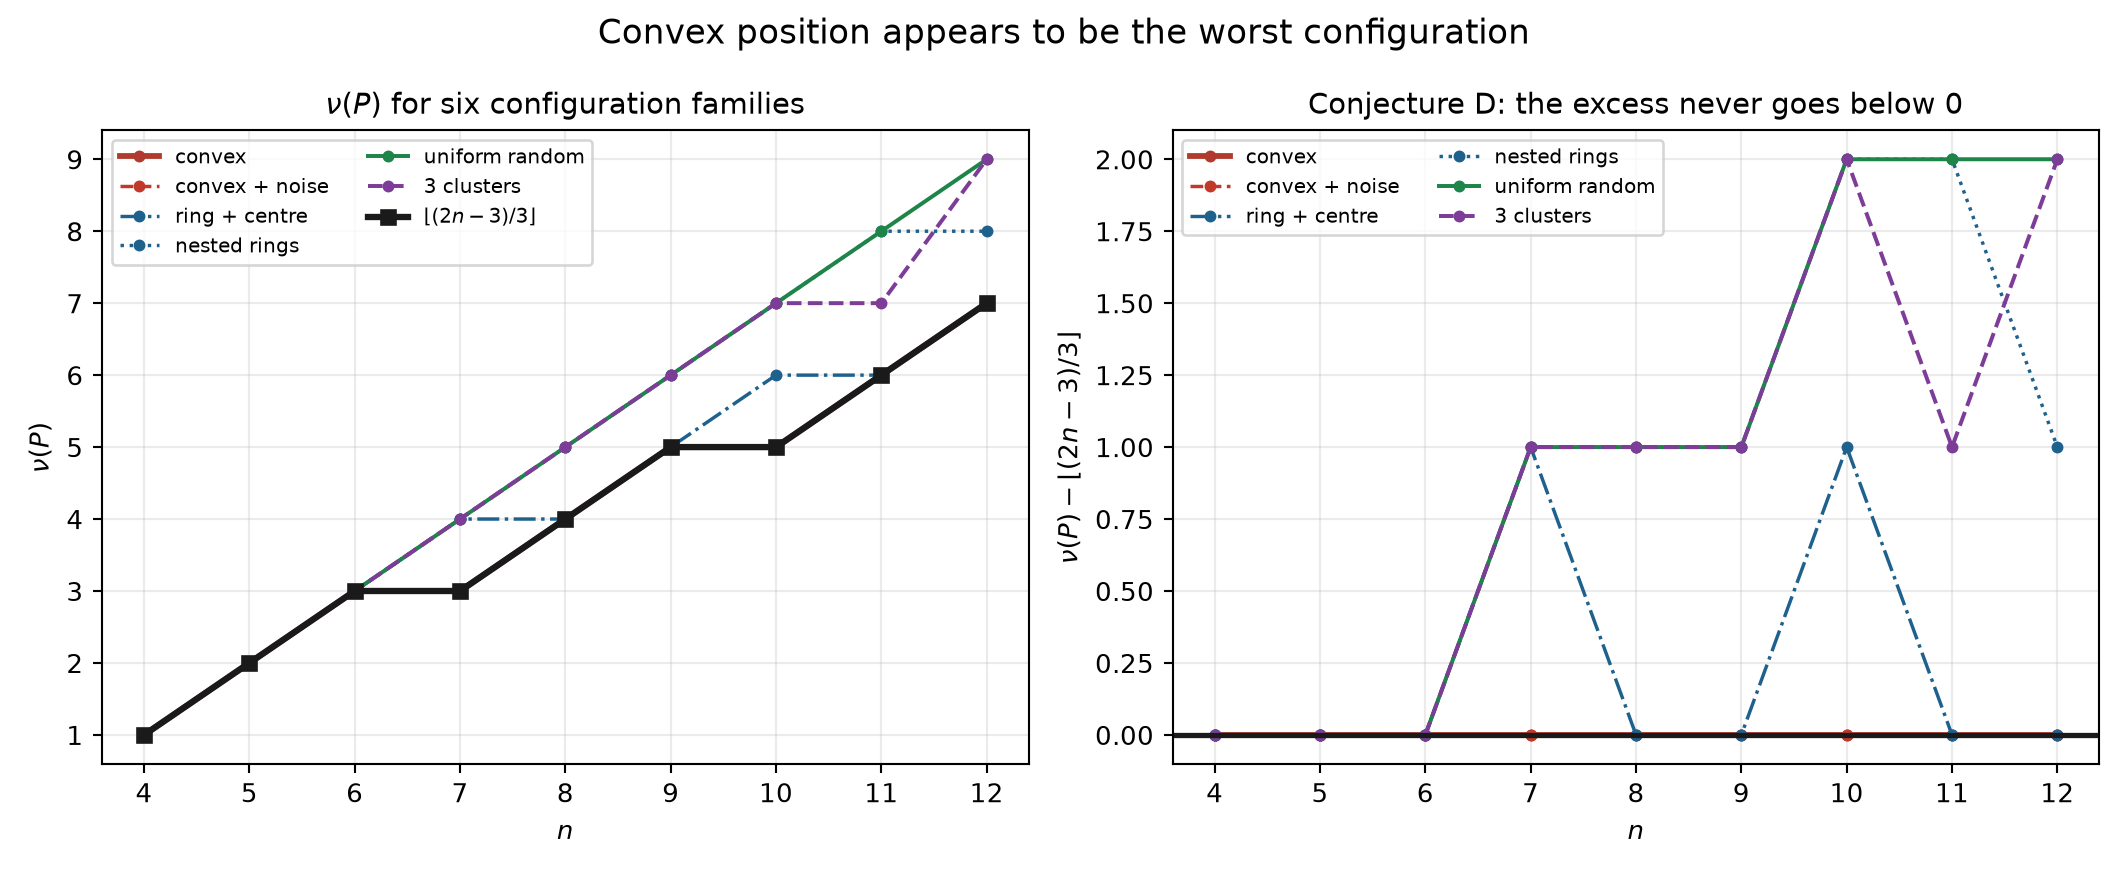
\includegraphics[width=\textwidth]{../figures/fig_configurations.png}
\caption{Left: $\nu(P)$ for six families of configurations.  Right: the excess
$\nu(P)-\Floor{(2n-3)/3}$.  Convex position is the only family attaining excess $0$ at
every $n$ in this sample, and no family dips below $0$.  This is evidence for
Conjecture~\ref{conj:barrier}, not a proof of it.}
\label{fig:configurations}
\end{figure}

\begin{figure}[t]
\centering
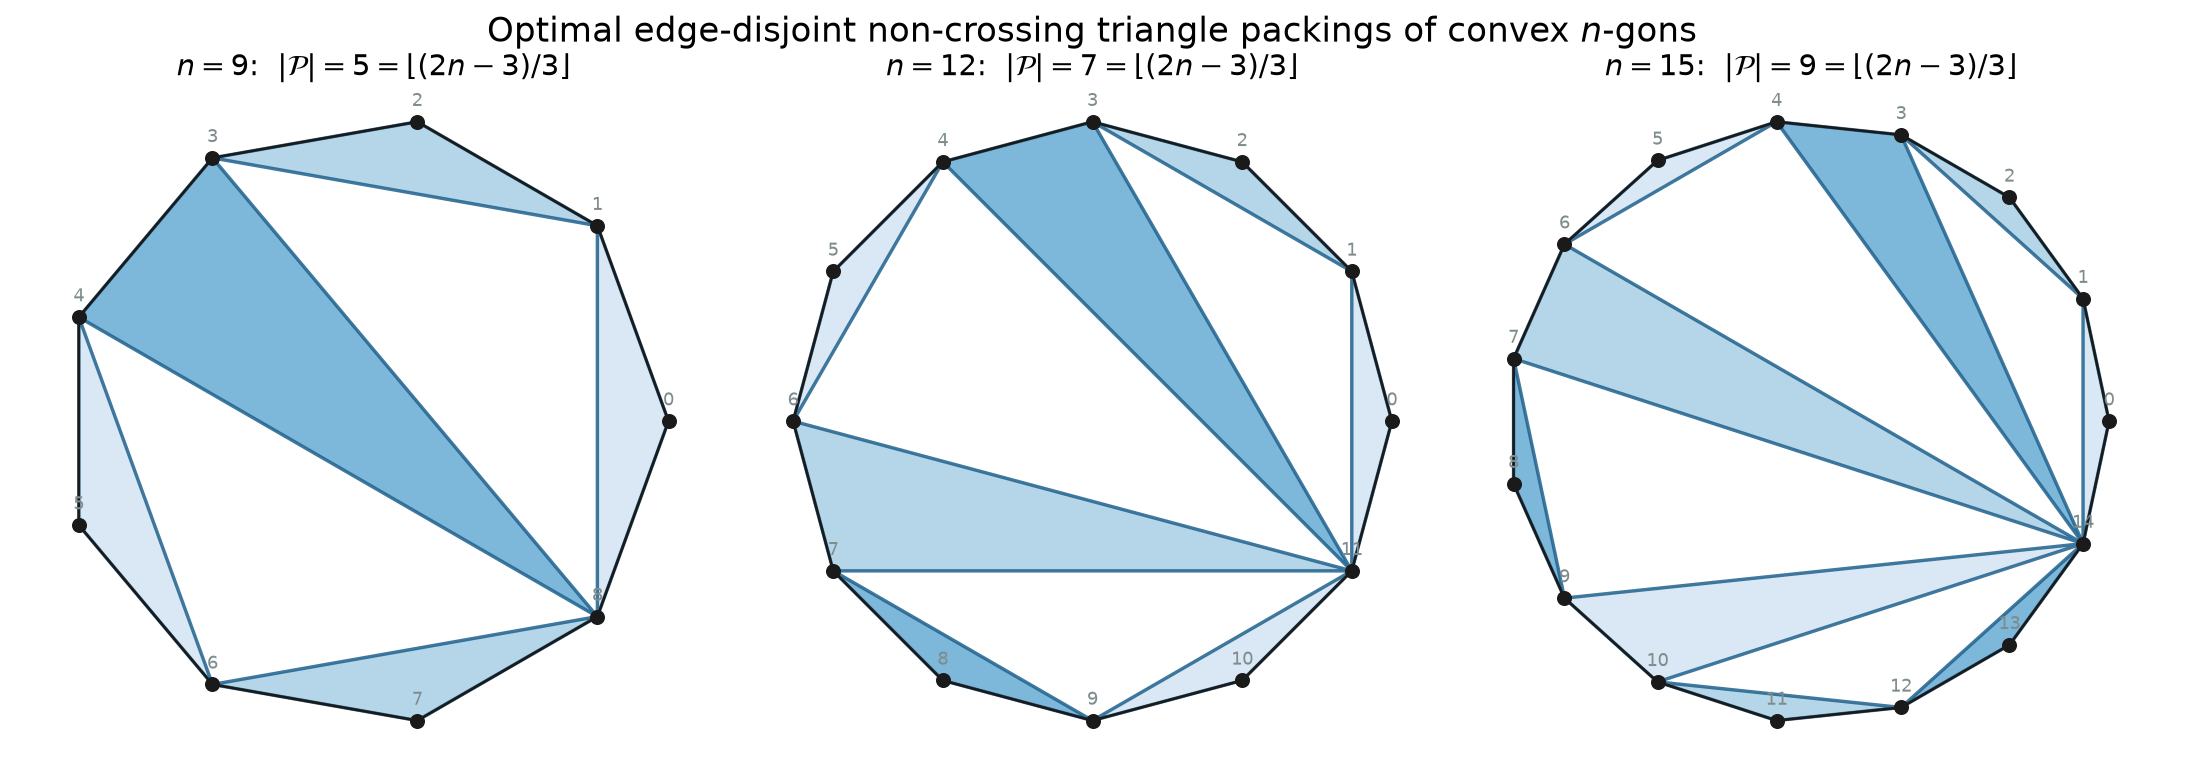
\includegraphics[width=0.95\textwidth]{../figures/fig_convex_packings.png}
\caption{Optimal packings produced by backtracking through recurrence
\eqref{eq:rec2}, for $n=9,12,15$.  Each has exactly $\Floor{(2n-3)/3}$ shaded triangles,
no two sharing an edge and no two with crossing edges.}
\label{fig:convex}
\end{figure}

\begin{figure}[t]
\centering
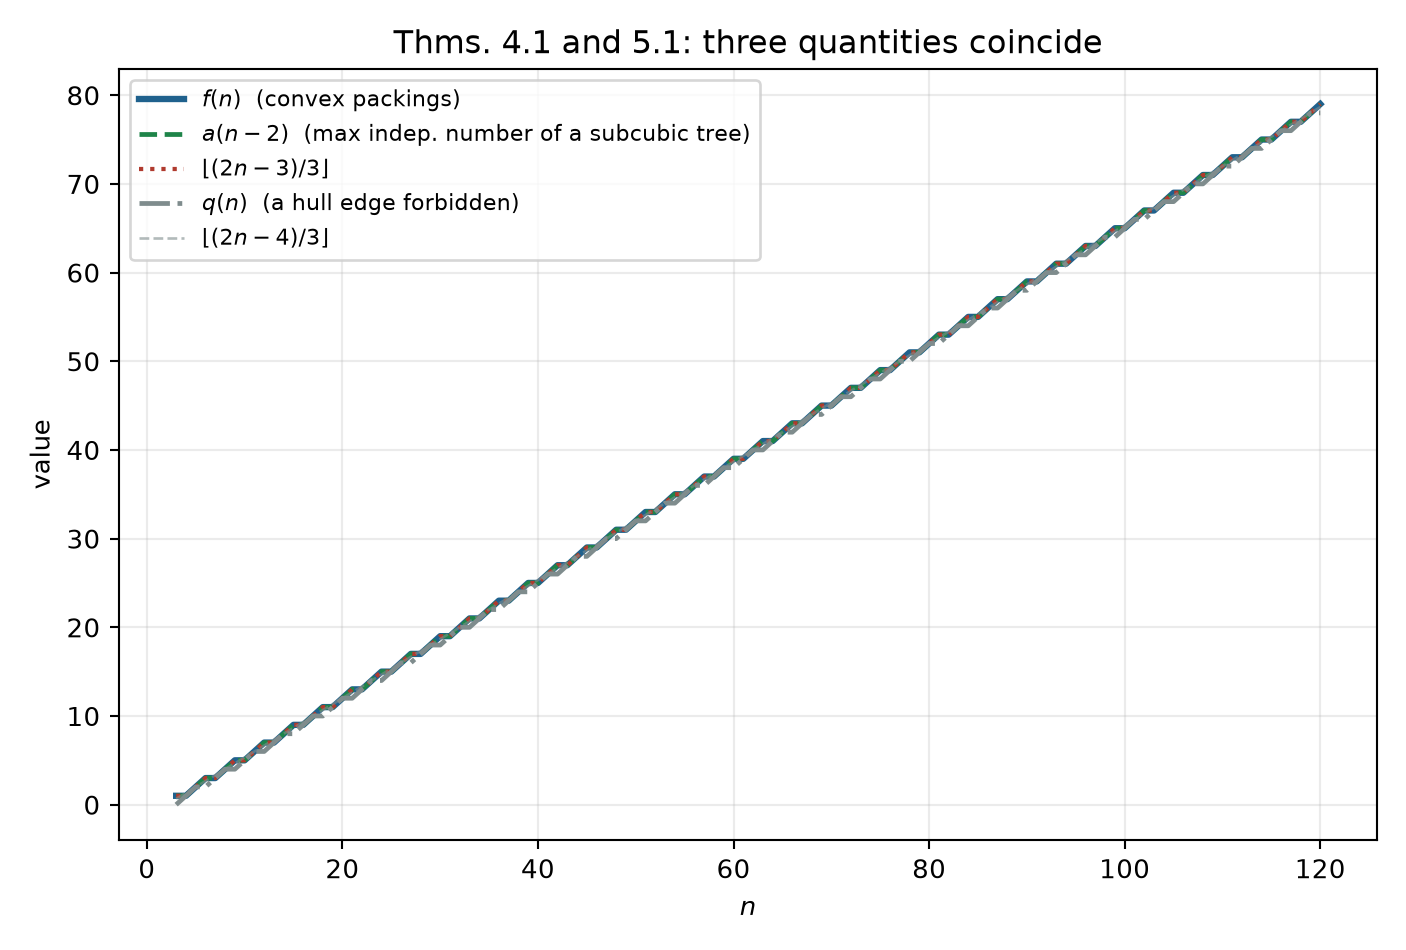
\includegraphics[width=\textwidth]{../figures/fig_three_functions.png}
\caption{The three quantities of Theorem~\ref{thm:a} coincide: the convex extremal
function $f(n)$, the maximum independence number $a(n-2)$ of a subcubic tree, and the closed
form $\Floor{(2n-3)/3}$.  Also shown is $q(n)$, the optimum when one hull edge is
forbidden.}
\label{fig:three}
\end{figure}

\begin{figure}[t]
\centering
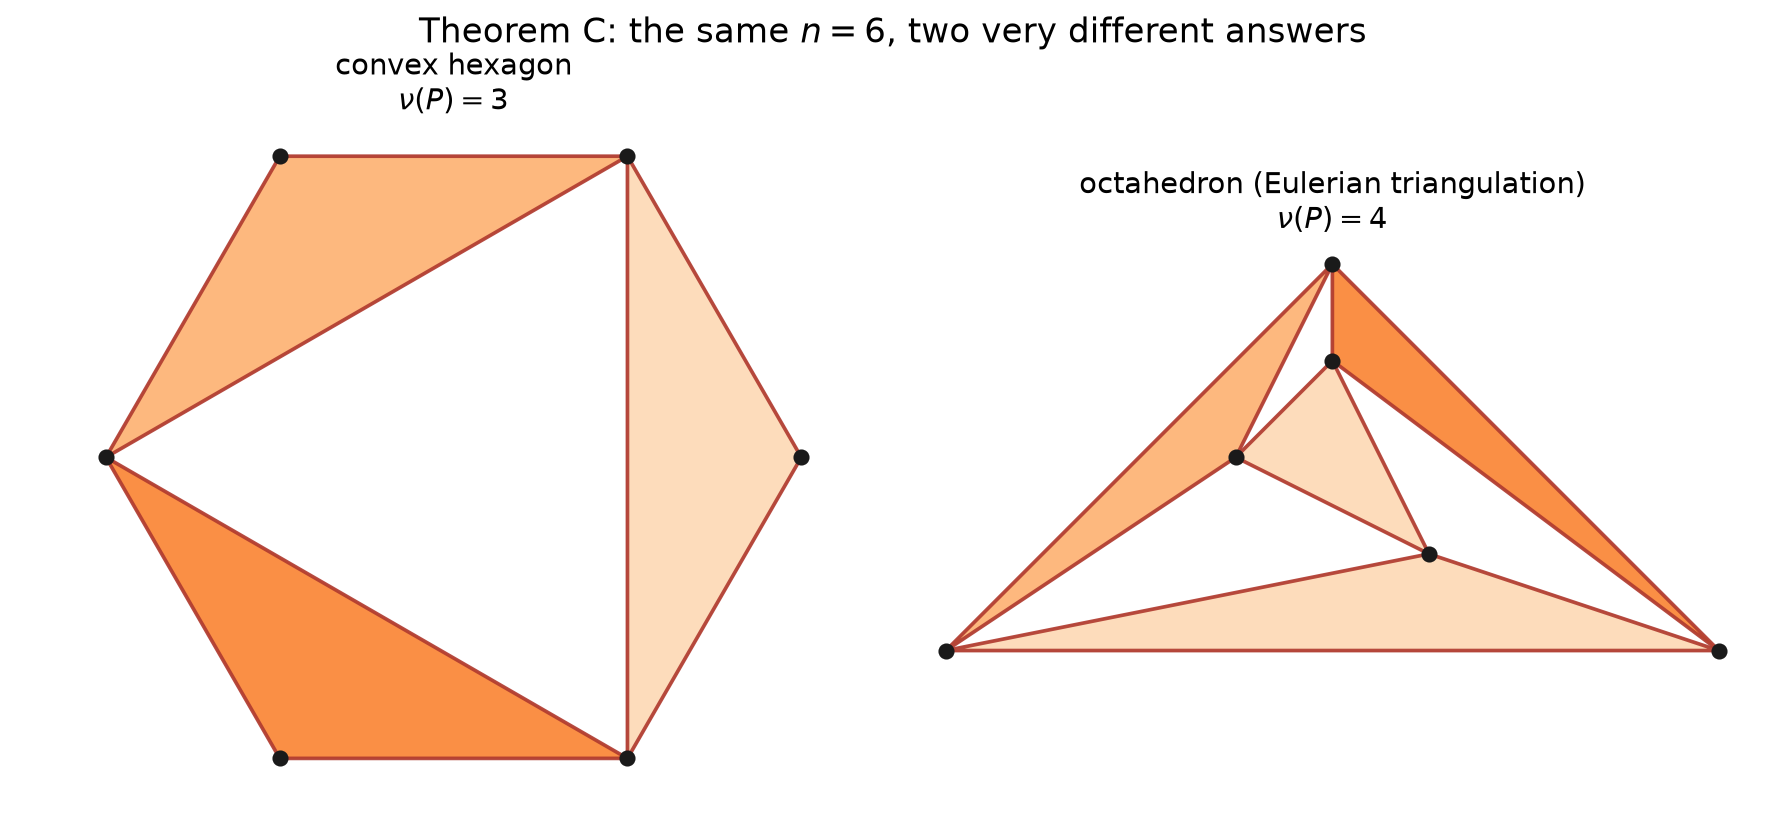
\includegraphics[width=0.8\textwidth]{../figures/fig_extremal_gap.png}
\caption{The same $n=6$, two answers.  Left: a convex hexagon supports
$\nu=3=\Floor{(2n-3)/3}$.  Right: a straight-line drawing of the octahedron supports
$\nu=4=n-2$.}
\label{fig:gap}
\end{figure}

\section{Computational cost of the experiments}

Running times are reported on a single core so that the experiments can be reproduced in
reasonable time.  These are measurements, not complexity-theoretic claims about the
underlying problems.

\begin{itemize}
\item \textbf{Convex extremal function.}  Recurrence \eqref{eq:rec2} is evaluated in
$O(n^2)$ time and $O(n)$ memory; backtracking a packing costs $O(n^2)$.  Lemma~\ref{lem:a}
makes the value itself available in $O(1)$.  The code computes the recurrence up to $n=400$
and compares with the closed form at every step.
\item \textbf{Subcubic trees.}  The independence number of an explicit tree is computed in
$O(N)$ time.  The exact maximum $a(N)$ is computed by a max-plus convolution in $O(N^3)$
time.
\item \textbf{Exhaustive triangulation scan.}  Triangulations of the convex $n$-gon are
$C_{n-2}$, so scanning all of them and computing an independent set of each weak dual
costs $O(C_{n-2}\,n)$; we do this for $n\le 10$ ($C_8=1430$).
\item \textbf{Exact packings on arbitrary point sets.}  We reduce $\nu(P)$ to maximum
independent set in the conflict graph on the $\binom n3$ triangles and solve
\[
\max\sum_T x_T \quad\text{s.t.}\quad x_S+x_T\le 1 \ \ \text{for every conflicting pair},
\qquad x_T\in\{0,1\},
\]
with HiGHS \cite{huangfuhall2018} through \texttt{scipy.optimize.milp}.  The program has
$\binom n3$ binary variables and $O(n^4)$ constraints; we solve it exactly for $n\le 12$.
\item \textbf{Maximal planar graph scan.}  Enumerating all labelled maximal planar graphs
on $n$ vertices means testing $\binom{\binom n2}{3n-6}$ candidate graphs for planarity;
$n=7$ is about $10^5$ candidates and takes a few minutes.
\end{itemize}

\section{Limitations and open problems}

\begin{enumerate}
\item \textbf{Conjecture~\ref{conj:barrier} is unproved.}  We verified it on $423$
configurations for $n\le 11$ (eleven structured families, exact integer programming) and on
the families of Figure~\ref{fig:configurations} for $n\le 12$.  A finite search is not a
proof, and the second assertion, that equality forces convex position, is supported only
computationally.
\item \textbf{The converse in Theorem~\ref{thm:general}} ($\nu=n-2$ forces an Eulerian
maximal planar graph) is verified for $n\le 7$ and is not proved in general; see
Remark~\ref{rem:honest}.
\item \textbf{The convex value is a counting bound.}  The upper bound
$\Floor{(2n-3)/3}$ is a two-line count, so the content of Part 1 is the construction and
the identification $f(n)=a(n-2)$, not the value itself.
\item \textbf{No variants.}  We did not investigate convex $k$-gons in place of triangles,
weighted versions, or the effect of allowing triangle interiors to overlap.
\end{enumerate}

\section{Conclusion}

We determined the largest number of pairwise non-crossing, edge-disjoint triangles spanned
by $n$ points in convex position: $\Floor{(2n-3)/3}$.  More interestingly, this geometric
extremal function coincides, term by term, with the maximum independence number of a
subcubic tree on $n-2$ vertices, itself equal to $\Floor{(2N+1)/3}$; the two ingredients are
that every $3$-cycle of a convex-polygon triangulation bounds a face, and that every
subcubic tree occurs as such a weak dual.  For arbitrary point sets we proved the sharp
bound $\nu(P)\le n-2$ and determined which $n$ admit extremal configurations, via Eulerian
triangulations and a complete existence classification.  What remains open here is whether
convex position is the worst configuration; we state it precisely as
Conjecture~\ref{conj:barrier} and report our unsuccessful attempts to prove it.

\begin{thebibliography}{9}

\bibitem{aichholzer2017}
O.~Aichholzer, T.~Hackl and M.~Korman, ``Packing plane spanning trees and paths in
complete geometric graphs,'' \textit{Information Processing Letters} \textbf{124} (2017),
35--41.

\bibitem{bernhartkainen1979}
F.~Bernhart and P.~Kainen, ``The book thickness of a graph,'' \textit{Journal of
Combinatorial Theory, Series B} \textbf{27} (1979), 320--331.

\bibitem{furedijiangkostochka2020}
Z.~F\"uredi, T.~Jiang and A.~V.~Kostochka, ``Extremal problems for convex geometric
hypergraphs and ordered hypergraphs,'' \textit{Canadian Journal of Mathematics}
\textbf{73} (2021), 1648--1666.

\bibitem{huangfuhall2018}
Q.~Huangfu and J.~A.~J.~Hall, ``Parallelizing the dual revised simplex method,''
\textit{Mathematical Programming Computation} \textbf{10} (2018), 119--142.

\bibitem{oneillspiro2021}
J.~O'Neill and S.~Spiro, ``Saturation problems in convex geometric hypergraphs,''
arXiv:2109.09931 (2021).

\bibitem{stanleyec2}
R.~P.~Stanley, \emph{Enumerative Combinatorics}, Volume 2, 2nd~ed., Cambridge University
Press, 2011.

\end{thebibliography}

\appendix

\section{Reproduction}

All experiments are deterministic.  From a clean clone:
\begin{verbatim}
pip install -e .
python -m pytest tests -q
python experiments/run_all.py
python experiments/make_figures.py
\end{verbatim}
Individual experiments, in increasing cost:
\begin{verbatim}
python experiments/exp1_convex.py     # f(n): DP and full enumeration, n<=10
python experiments/exp3_weakdual.py   # structural lemmas, exhaustively
python experiments/exp2_falsify.py    # Conjecture 7.1: hunt for counterexamples
python experiments/exp4_general.py    # Theorem 6.5: all maximal planar graphs, n<=7
\end{verbatim}
The scan of all maximal planar graphs for $n=7$ takes a few minutes; set the environment
variable \texttt{PLANETRI\_MAX\_ENUM\_N=6} to shorten it.

\section{Where the code lives}

\begin{center}\small
\begin{tabular}{@{}l@{}}
\texttt{src/planetri/geom.py}\\[-2pt]
\quad exact orientation and crossing predicates on exact points\\[4pt]
\texttt{src/planetri/solver.py}\\[-2pt]
\quad conflict graph and exact maximiser via 0/1 programming\\[4pt]
\texttt{src/planetri/convex.py}\\[-2pt]
\quad recurrence \eqref{eq:rec2}, closed form, constructive packings\\[4pt]
\texttt{src/planetri/trees.py}\\[-2pt]
\quad independence numbers of subcubic trees, weak duals\\[4pt]
\texttt{tests/test\_planetri.py}\\[-2pt]
\quad the test suite
\end{tabular}
\end{center}

\end{document}